%%%%%%%%%%%%%%%%%%%%%%%%%%%%%%%%%%%%%%%%%
% Beamer Presentation
% LaTeX Template
% Version 1.0 (10/11/12)
%
% This template has been downloaded from:
% http://www.LaTeXTemplates.com
%
% License:
% CC BY-NC-SA 3.0 (http://creativecommons.org/licenses/by-nc-sa/3.0/)
%
%%%%%%%%%%%%%%%%%%%%%%%%%%%%%%%%%%%%%%%%%

%----------------------------------------------------------------------------------------
%	PACKAGES AND THEMES
%----------------------------------------------------------------------------------------

\documentclass[aspectratio=149]{beamer}
\usefonttheme[onlymath]{serif}


\mode<presentation> {

% The Beamer class comes with a number of default slide themes
% which change the colors and layouts of slides. Below this is a list
% of all the themes, uncomment each in turn to see what they look like.

\usetheme{default}
%\usetheme{AnnArbor}
%\usetheme{Antibes}
%\usetheme{Bergen}
%\usetheme{Berkeley}
%\usetheme{Berlin}
%\usetheme{Boadilla}
%\usetheme{CambridgeUS}
%\usetheme{Copenhagen}
%\usetheme{Darmstadt}
%\usetheme{Dresden}
%\usetheme{Frankfurt}
%\usetheme{Goettingen}
%\usetheme{Hannover}
%\usetheme{Ilmenau}
%\usetheme{JuanLesPins}
%\usetheme{Luebeck}
%\usetheme{Malmoe}
%\usetheme{Marburg}
%\usetheme{Montpellier}
%\usetheme{PaloAlto}
%\usetheme{Pittsburgh}
%\usetheme{Rochester}
%\usetheme{Singapore}
%\usetheme{Szeged}
%\usetheme{Warsaw}

% As well as themes, the Beamer class has a number of color themes
% for any slide theme. Uncomment each of these in turn to see how it
% changes the colors of your current slide theme.

%\usecolortheme{albatross}
\usecolortheme{beaver}
%\usecolortheme{beetle}
%\usecolortheme{crane}
%\usecolortheme{dolphin}
%\usecolortheme{dove}
%\usecolortheme{fly}
%\usecolortheme{lily}
%\usecolortheme{orchid}
%\usecolortheme{rose}
%\usecolortheme{seagull}
%\usecolortheme{seahorse}
%\usecolortheme{whale}
%\usecolortheme{wolverine}

%\setbeamertemplate{footline} % To remove the footer line in all slides uncomment this line
%\setbeamertemplate{footline}[page number] % To replace the footer line in all slides with a simple slide count uncomment this line

%\setbeamertemplate{navigation symbols}{} % To remove the navigation symbols from the bottom of all slides uncomment this line
}

\usepackage{graphicx} % Allows including images
\usepackage{booktabs} % Allows the use of \toprule, \midrule and \bottomrule in tables
\usepackage{verbatim}

\usepackage{mathtools} 
\usepackage{amssymb}
\usepackage{mathrsfs}
\usepackage{amsmath}
\usepackage{bm}

\usepackage{ragged2e}
\usepackage{etoolbox}
\usepackage{lipsum}

\usepackage{siunitx,booktabs}
\usepackage{pifont}
\usepackage{array}
\usepackage{tabu,booktabs}
\usepackage{tikz}
\usetikzlibrary{arrows,shapes}

\setbeamertemplate{enumerate items}[circle]
\usepackage{tikz}

\usepackage{dsfont}

\definecolor{manatee}{rgb}{0.59, 0.6, 0.67}
\definecolor{gr}{gray}{0.23}
\definecolor{navyblue}{rgb}{0.0, 0.0, 0.5}
\definecolor{lincolngreen}{rgb}{0.11, 0.35, 0.02}
\definecolor{copper}{rgb}{0.72, 0.45, 0.2}
\definecolor{darkorange}{rgb}{1.0, 0.55, 0.0}
\definecolor{darkpowderblue}{rgb}{0.0, 0.2, 0.6}
\definecolor{darksienna}{rgb}{0.24, 0.08, 0.08}
\definecolor{darkred}{rgb}{0.55, 0.0, 0.0}

\newcommand\mynum[1]{
  \usebeamercolor{enumerate item}
  \tikzset{beameritem/.style={circle,inner sep=0,minimum size=2ex,text=enumerate item.bg,fill=enumerate item.fg,font=\footnotesize}}%
  \tikz[baseline=(n.base)]\node(n)[beameritem]{#1};
}

\newcommand\mynumm[1]{
  \usebeamercolor{enumerate item}
  \tikzset{beameritem/.style={rectangle,inner sep=0,minimum size=2ex,text=enumerate item.bg,fill=enumerate item.fg,font=\footnotesize}}%
  \tikz[baseline=(n.base)]\node(n)[beameritem]{#1};
}

\def\Put(#1,#2)#3{\leavevmode\makebox(0,0){\put(#1,#2){#3}}}

\setbeamertemplate{footline}[]

%----------------------------------------------------------------------------------------
%	TITLE PAGE
%----------------------------------------------------------------------------------------

\title{Urban Water and Housing Infrastructure  \\ for Economic Development} % The short title appears at the bottom of every slide, the full title is only on the title page

\author{William Violette} 

 % Your institution as it will appear on the bottom of every slide, may be shorthand to save space

\date{May 2018} %\today} % Date, can be changed to a custom date

\begin{document}

\beamertemplatenavigationsymbolsempty

\begin{frame}
\titlepage % Print the title page as the first slide
\end{frame}

%\begin{frame}
%\frametitle{Overview} % Table of contents slide, comment this block out to remove it
%\tableofcontents % Throughout your presentation, if you choose to use \section{} and \subsection{} commands, these will automatically be printed on this slide as an overview of your presentation
%\end{frame}


%------------------------------------------------

%\begin{frame}
%\frametitle{Slums and Development}
%\begin{tabular}{lc} \hline
 & (1) \\
VARIABLES & Log Price \\ \hline
 &  \\
3 yrs 0-400m & -0.125 \\
 & (0.0892) \\
3 yrs 0-400m X In-Situ & 0.180 \\
 & (0.289) \\
 &  \\
Observations & 28,701 \\
R-squared & 0.489 \\
Project FE & YES \\
 Year-Month FE & YES \\ \hline
\multicolumn{2}{c}{ Robust standard errors in parentheses} \\
\multicolumn{2}{c}{ *** p$<$0.01, ** p$<$0.05, * p$<$0.1} \\
\multicolumn{2}{c}{ All control for cubic in plot size. Standard errors are clustered at the project level.} \\
\end{tabular}

%\end{frame}

%----------------------------------------------------------------------------------------
%	PRESENTATION SLIDES
%----------------------------------------------------------------------------------------


\begin{frame}
\frametitle{Motivation for Dissertation}
\begin{itemize}
  \item Rapid urbanization in the developing world
    \begin{itemize}
      \item  30\% of urban pop. lives in slums (UN, 2015)
    \end{itemize}
\vspace{.2cm}
  \item Informal institutions mean standard policies can have unintended consequences
  \begin{itemize}
    \item Difficult to detect in standard survey data
  \end{itemize}
\vspace{.2cm}
  \item New administrative data can provide a window into these dynamics
\end{itemize}
\end{frame}





\begin{frame}
\frametitle{Overview of Dissertation}

\begin{enumerate}
\item Spillover impacts of public housing
\item Child health, overcrowding, and public housing
\item Pricing water when the poor share
\end{enumerate}
\end{frame}





\begin{frame}
\frametitle{}
\centering
{\Large \color{darkred} Public Housing Spillovers \\ in a Developing Country } \\
\vspace{.4cm}
joint with Ben Bradlow and Stefano Polloni
\end{frame}



\begin{frame}
\frametitle{Public Housing and Development}

% In developing countries, 30\% of urban pop live in slums (UN, 2015)

\begin{itemize}
  \item Public Housing $\rightarrow$ primary government response to slums
  \vspace{.1cm}
  \item Positive effects on direct recipients \\ 
  {\footnotesize (Cateneo et al. [2009], Franklin et al. [2016], Galiani et al. [2017])}
  \vspace{.1cm}
  \item \textbf{Question:}  What are the spillover effects of public housing in developing countries?
      \begin{itemize}
      \item \textit{Positive:} Amenity value
      \item \textit{Negative:} Crowd-in slums (share public services)
    \end{itemize}
  \vspace{.1cm}
  \item \textbf{Setting:} 150+ projects in South Africa; GPS price and slum data
  \vspace{.1cm}
  \item \textbf{Findings:} Home prices drop by 16\% within 3 yrs and 400m of a project
    \begin{itemize}
      \item Home quality improves within project footprint but declines nearby (slum crowd-in)
    \end{itemize}
\end{itemize}
\end{frame}


%------------------------------------------------

\begin{frame}
\frametitle{Public Housing in South Africa}
  \begin{itemize}
      \item Over 4.3 million houses since 1994 (13\% of pop.)
%      \item Houses 13\% of the population
%      \item Single-story, two-room (30-40$\text{m}^2$) dwellings
      \begin{itemize}
        \item 50 to 500 houses per project
        \item Fully serviced (roads, water, sanitation, electricity)
        \item Greenfield projects on undeveloped land near slums
        \item In-Situ upgrading replacing existing slums
      \end{itemize}
     %     \begin{enumerate}
     %       \item \textbf{Greenfield projects} on undeveloped land near slums
     %       \item \textbf{In-Situ upgrading} replacing existing slums
     %     \end{enumerate}
    \vspace{.1cm}
    \item Who gets a house?
      \begin{itemize}
        \item National/provincial waiting list; no resale within 7 years
        \item Must be eligible: Citizens, new homeowners, married or dependents, low income
        \item In practice, waiting lists/eligibility weakly enforced
          %  \item Only 82\% of houses occupied by initial owners within 5 yrs
      \end{itemize}
  \end{itemize}
    %%% insert picture


\begin{center}
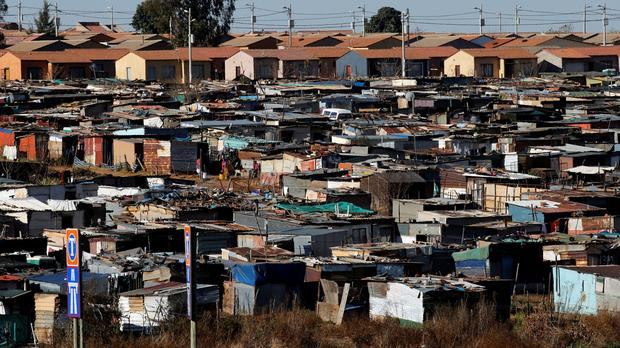
\includegraphics[scale=1]{slum_rdp.jpeg}
\end{center}

\end{frame}



%------------------------------------------------



\begin{frame}
\frametitle{Measuring Public Housing and Spillovers}

\begin{itemize}
  \item Focus on Gauteng Province (includes Johannesburg and Pretoria)
\end{itemize}

\begin{enumerate}
\item \textbf{Property Transactions} 500,000 deeds records (bottom 20\% of formal housing market)
  \begin{itemize}
    \item Buyer/seller name, GPS, price, date from 2002-2011
  \end{itemize}
\vspace{.1cm}
\item \textbf{Building Census:} GPS for over 4 mil. buildings in 2001 and 2011
\vspace{.1cm}
\item \textbf{Population Census:} 2001 and 2011
\vspace{.1cm}
\item \textbf{Admin. Project Records:} location, dates, costs
  \begin{itemize}
    \item Includes planned but unconstructed projects
  \end{itemize}
\end{enumerate}
\end{frame}

%------------------------------------------------

\begin{frame}
\frametitle{Identifying Housing Projects}
\label{data}
\textbf{Completed Projects:} 56
\begin{itemize}
\item Use sales from government sellers on previously empty land plots
\item Cluster sales into projects based on geographic proximity
\item Include projects where over 50\% of sales occurred in the same year
  \begin{itemize}
    \item Use modal sale year as project date
  \end{itemize}
\end{itemize}
\vspace{.4cm}
\textbf{Uncompleted Projects:} 101
\begin{itemize}
\item Admin. projects that do not overlap with completed projects
  \begin{itemize}
    \item Use estimated completion date as project date
  \end{itemize}
  \item Why are projects canceled/delayed? 
    \begin{itemize}
      \item Legal disputes, service delivery backlogs, funding complications
      \item Delays can exceed 12 years 
    \end{itemize} 
\end{itemize}
\hyperlink{dataappendix}{\beamerbutton{data appendix}}
\end{frame}

%------------------------------------------------
\begin{frame}
%\frametitle{Housing projects}
\vspace*{-18mm}
\begin{center}
\hspace*{-17mm}
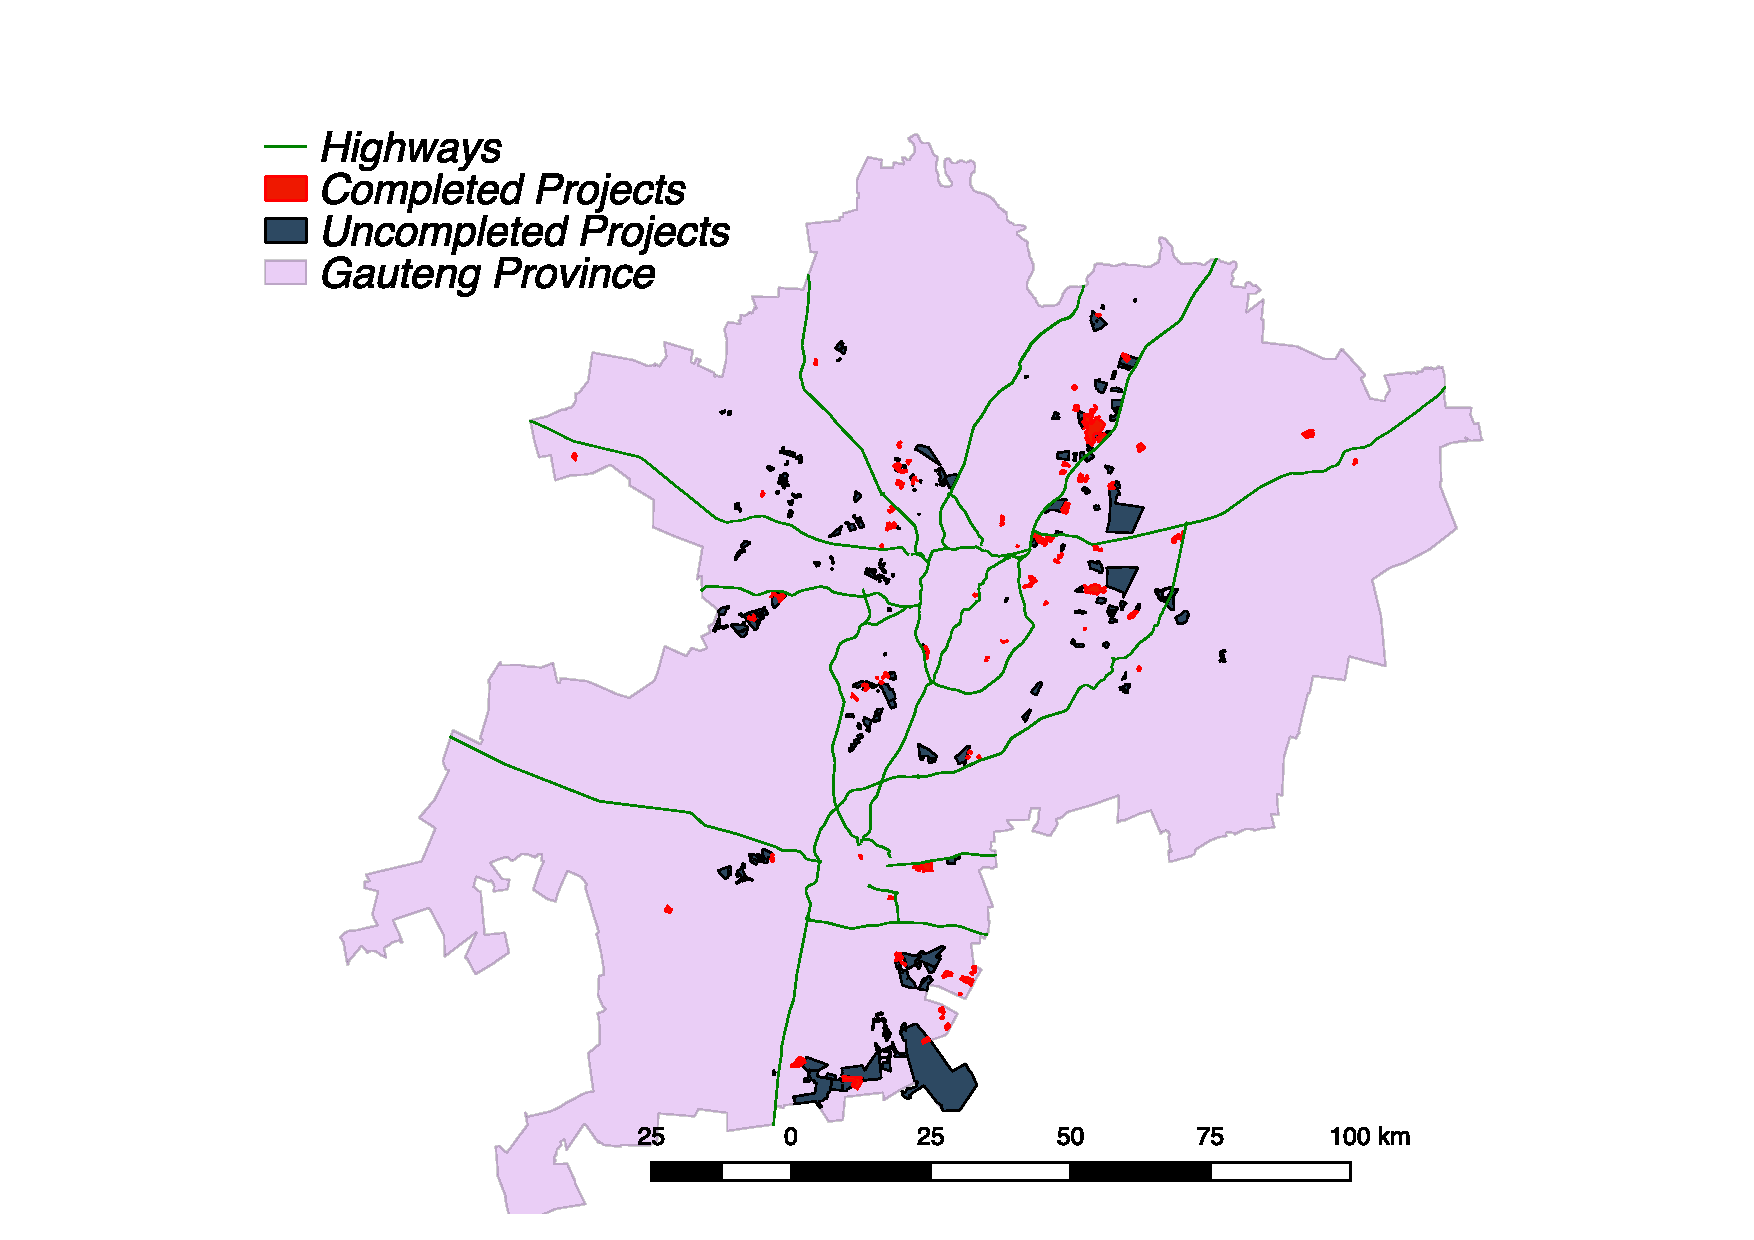
\includegraphics[scale=0.47]{full_map.pdf}
\vspace{-3mm}
\end{center}
\end{frame}

%\begin{frame}
% \frametitle{Housing Projects}
% \begin{center}
% \begin{tabu}{lcc}
 & Completed & Uncompleted \\ 
 Formal Density: 2001  & 340.6  & 89.1  \\ 
 Formal Density: 2011  & 1,783.1  & 491.1  \\ 
 &  &  \\ 
 Informal Density: 2001  & 443.0  & 1,569.2  \\ 
 Informal Density: 2011  & 1,064.6  & 1,993.4  \\ 
 &  &  \\ 
 Median Year (est.)  & 2005  & 2007  \\ 
 Distance to CBD (km)  & 28.9  & 27.6  \\ 
 &  &  \\ 
 Total Projects   & 56  & 35  \\ 
\bottomrule
\end{tabu}

% \end{center}
% Home counts are from building census.
% \end{frame}


%-------------------- BUILDING COUNTS --------------
\begin{frame}
\frametitle{How do projects affect housing growth?}
\begin{itemize}
  \item Count structures within 50 by 50 meter grids
\end{itemize}
\begin{center}
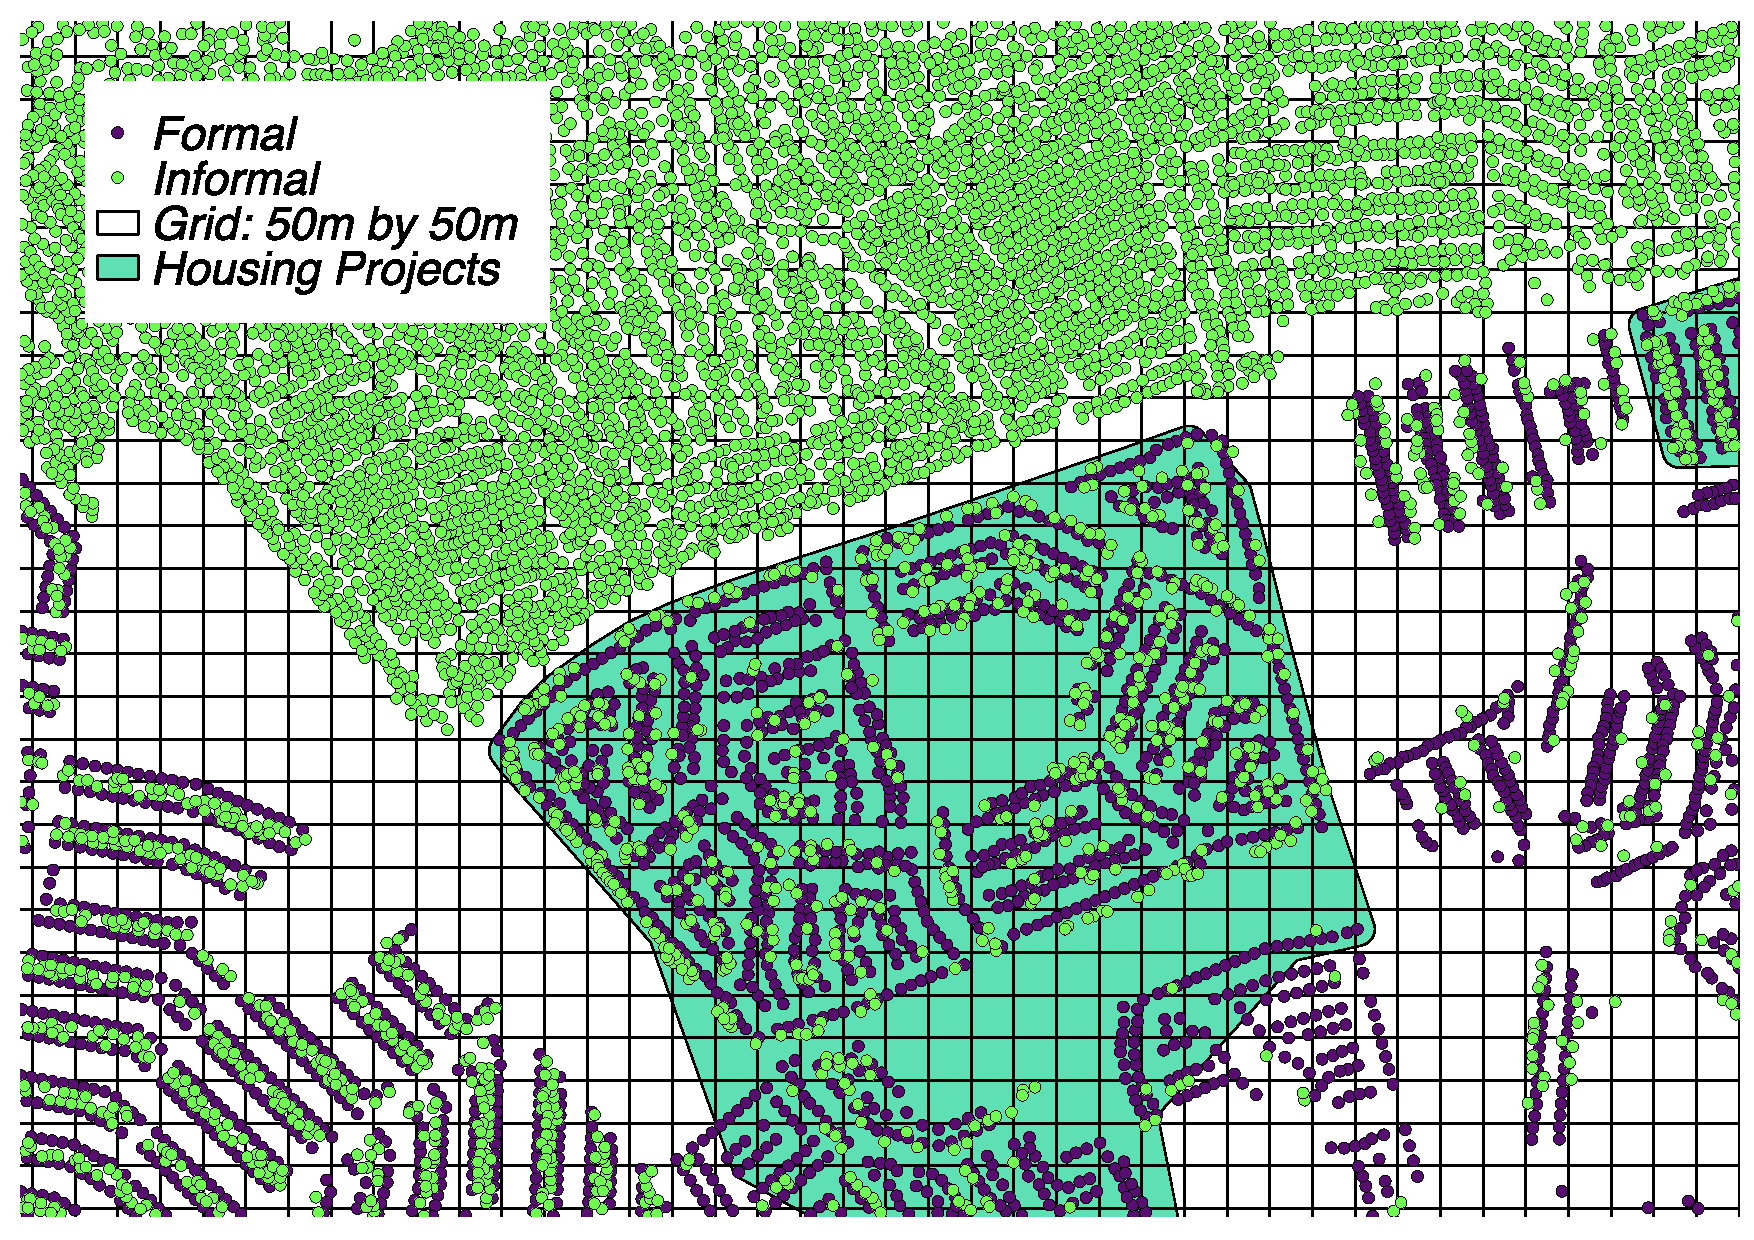
\includegraphics[scale=0.31]{bblu_map.pdf}\\
Post construction (2011)
\vspace{-3mm}
\end{center}
\end{frame}





%------------------------------------------------

%\begin{frame}
%\frametitle{Estimating Differences-in-Differences}
%
%\begin{align*}
%H_{gtp} \, &= \, \sum_{d=1}^{D} \alpha_d \mathds{1}[dist=d] Post_{tp} C_p + \sum_{d=1}^{D} \beta_d \%mathds{1}[dist=d] Post_{tp} U_p   \\
%& +  \lambda_g \, + \, \varepsilon_{gtp}
%\end{align*}
%
%\begin{itemize}
%\item $g$: grid cell, $t$: year (2001, 2011), $p$: project
%\item $H_{gtp}$: Houses per grid cell
%\item $dist$: distance from boundary ($<0$ within project)
%\item $Post_{tp}$: After project
%\item $C_{bp}$: Completed, $U_{bp}$: Uncompleted
%\item $\lambda_g$: grid cell fixed effect
%\end{itemize}
%
%\begin{itemize}
%  \item \textbf{Identification}: Counterfactual outcomes for completed projects would have changed in %the same way as uncompleted projects.
%\end{itemize}
%
%\end{frame}
%
%%------------------------------------------------

%\begin{frame}
%\frametitle{All Houses}
%\begin{center}
%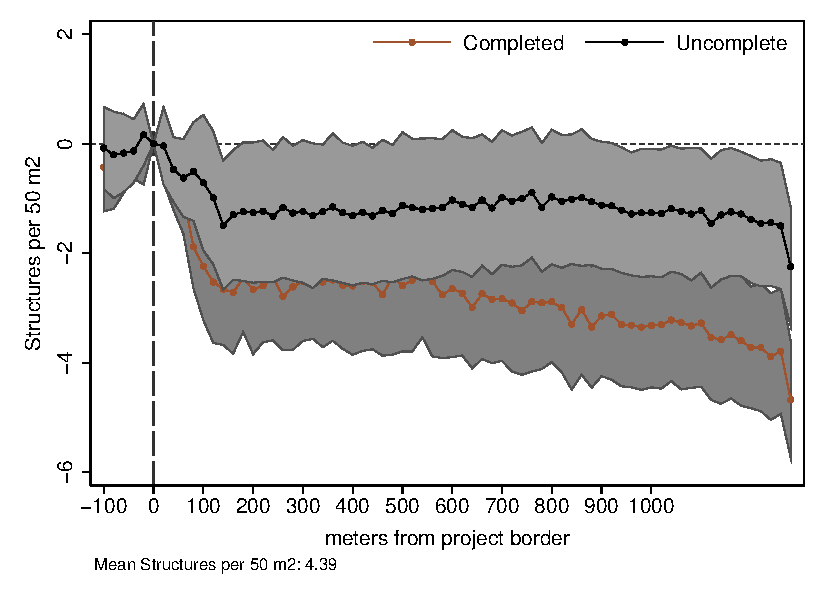
\includegraphics[scale=.78]{distplot_bblu_b.pdf}
%\vspace{-3mm}
%\end{center}
%\end{frame}

\begin{frame}
\frametitle{Formal Houses}
\hspace{10mm} Completed Projects \hspace{30mm} Uncompleted Projects
\hspace*{-10mm}
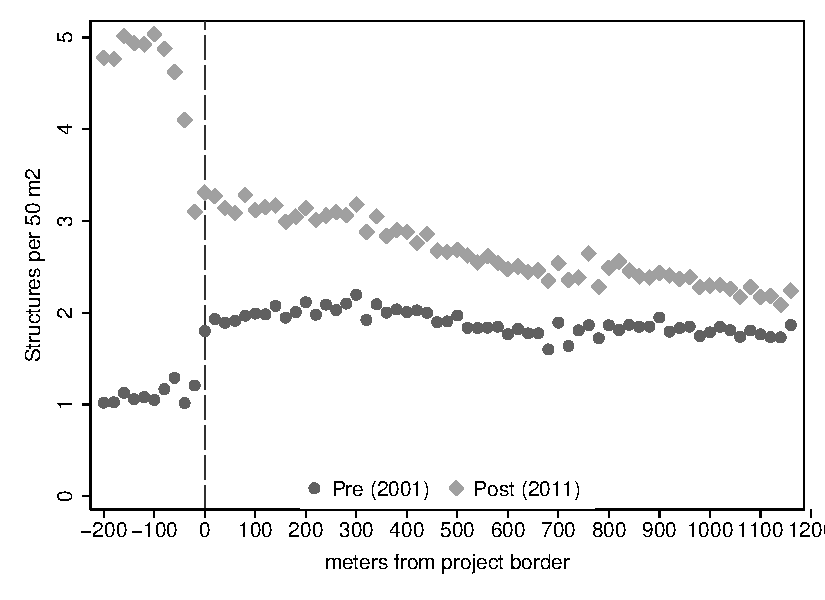
\includegraphics[scale=.48]{bblu_for_c.pdf}
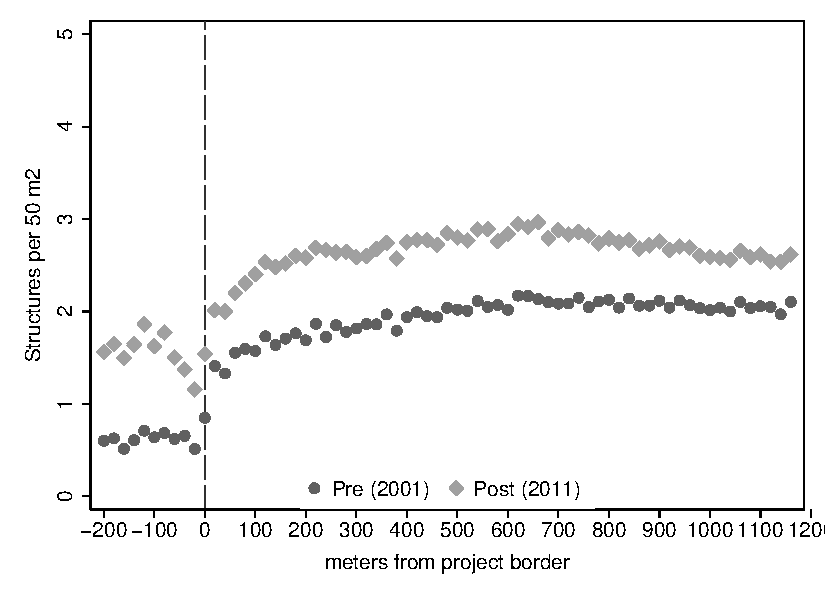
\includegraphics[scale=.48]{bblu_for_p.pdf}
\end{frame}

\begin{frame}
\frametitle{Change in Formal Houses}
\begin{center}
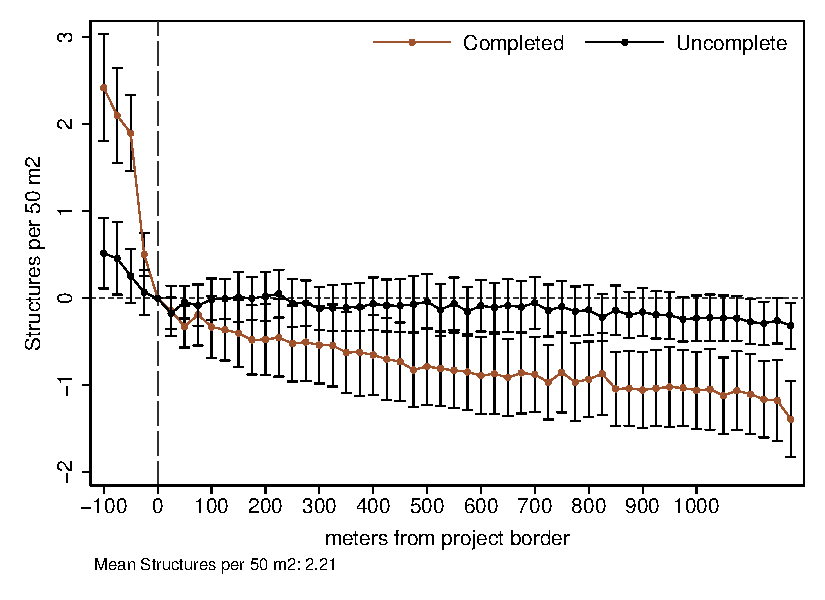
\includegraphics[scale=.78]{distplot_bblu_for.pdf}
\vspace{-3mm}
\end{center}
\end{frame}

\begin{frame}
\frametitle{Change in Informal Houses}
\hspace{10mm} Completed Projects \hspace{30mm} Uncompleted Projects
\hspace*{-10mm}
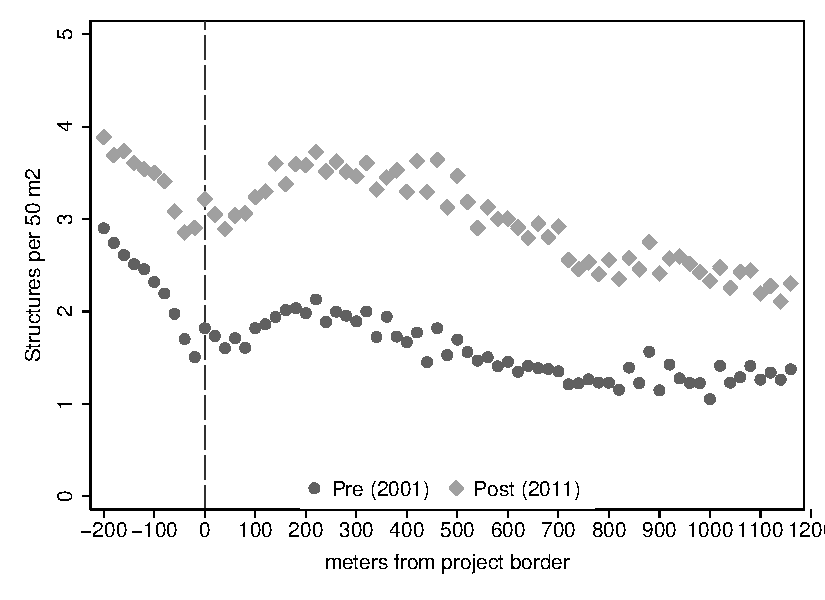
\includegraphics[scale=.48]{bblu_inf_c.pdf}
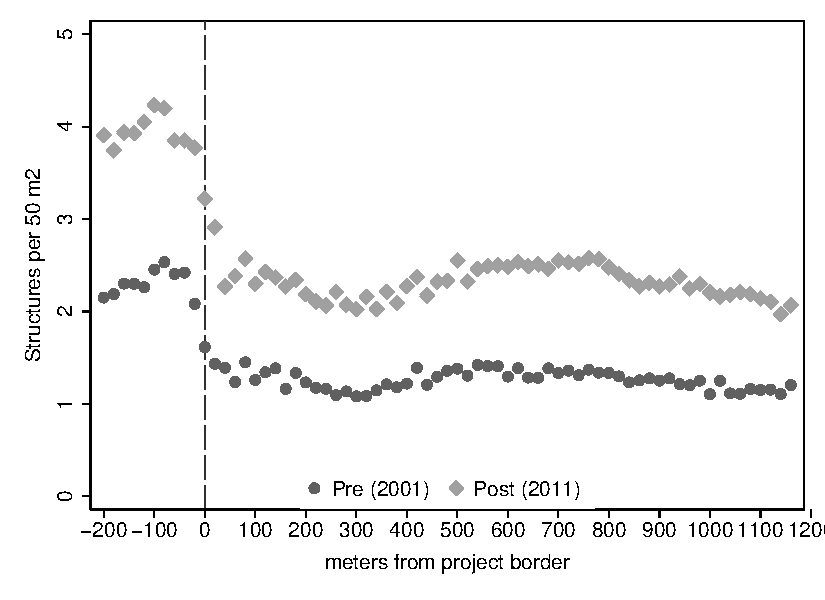
\includegraphics[scale=.48]{bblu_inf_p.pdf}
\end{frame}

\begin{frame}
\frametitle{Informal Houses (Slums)}
\begin{center}
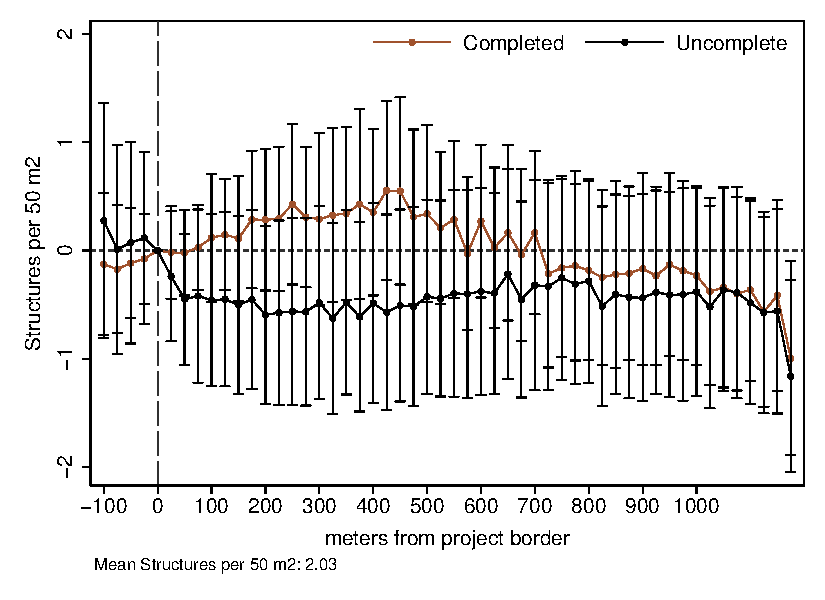
\includegraphics[scale=.78]{distplot_bblu_inf.pdf}
\vspace{-3mm}
\end{center}
\end{frame}


% \begin{frame}
% \frametitle{Shops}
% \hspace{10mm} Completed Projects \hspace{30mm} Uncompleted Projects
% \hspace*{-10mm}
% 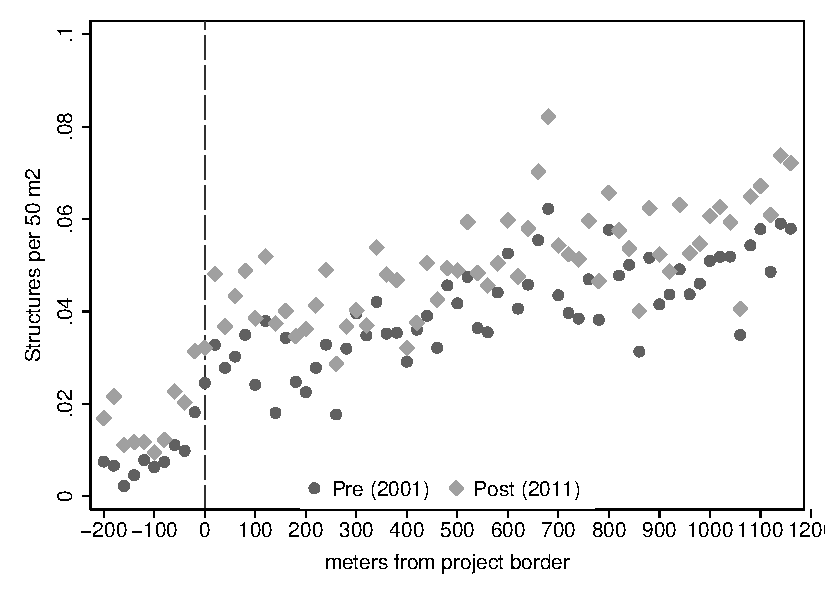
\includegraphics[scale=.48]{bblu_shops_c.pdf}
% 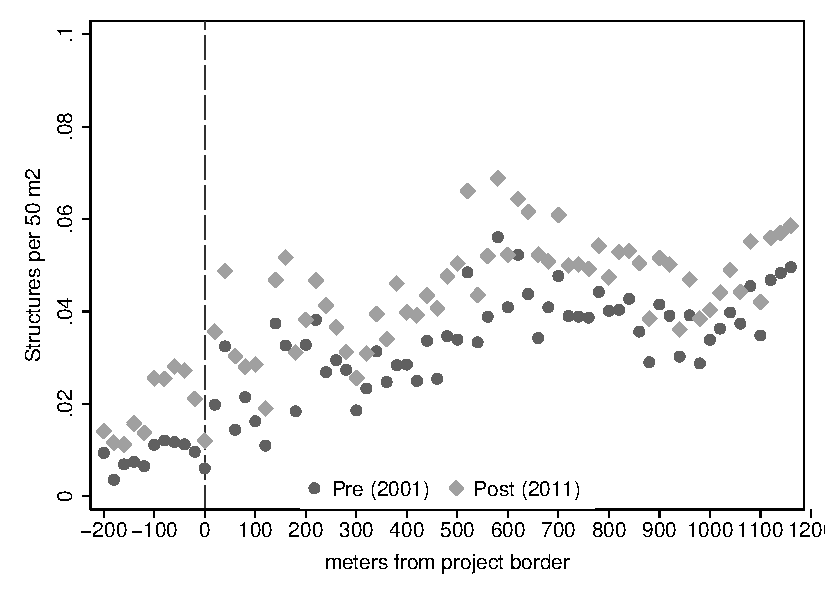
\includegraphics[scale=.48]{bblu_shops_p.pdf}
% \end{frame}



%---------------------  CENSUS EFFECTS  ---------------------------

\begin{frame}
\frametitle{How do projects affect census demographics and house quality?}
\begin{itemize}
  \item Project Blocks: $>$30\% overlap (yellow)
  \item Spillover Blocks: $<$30\% overlap, centroids within 1.2 km (blue)
\end{itemize}
\begin{center}
\begin{figure}
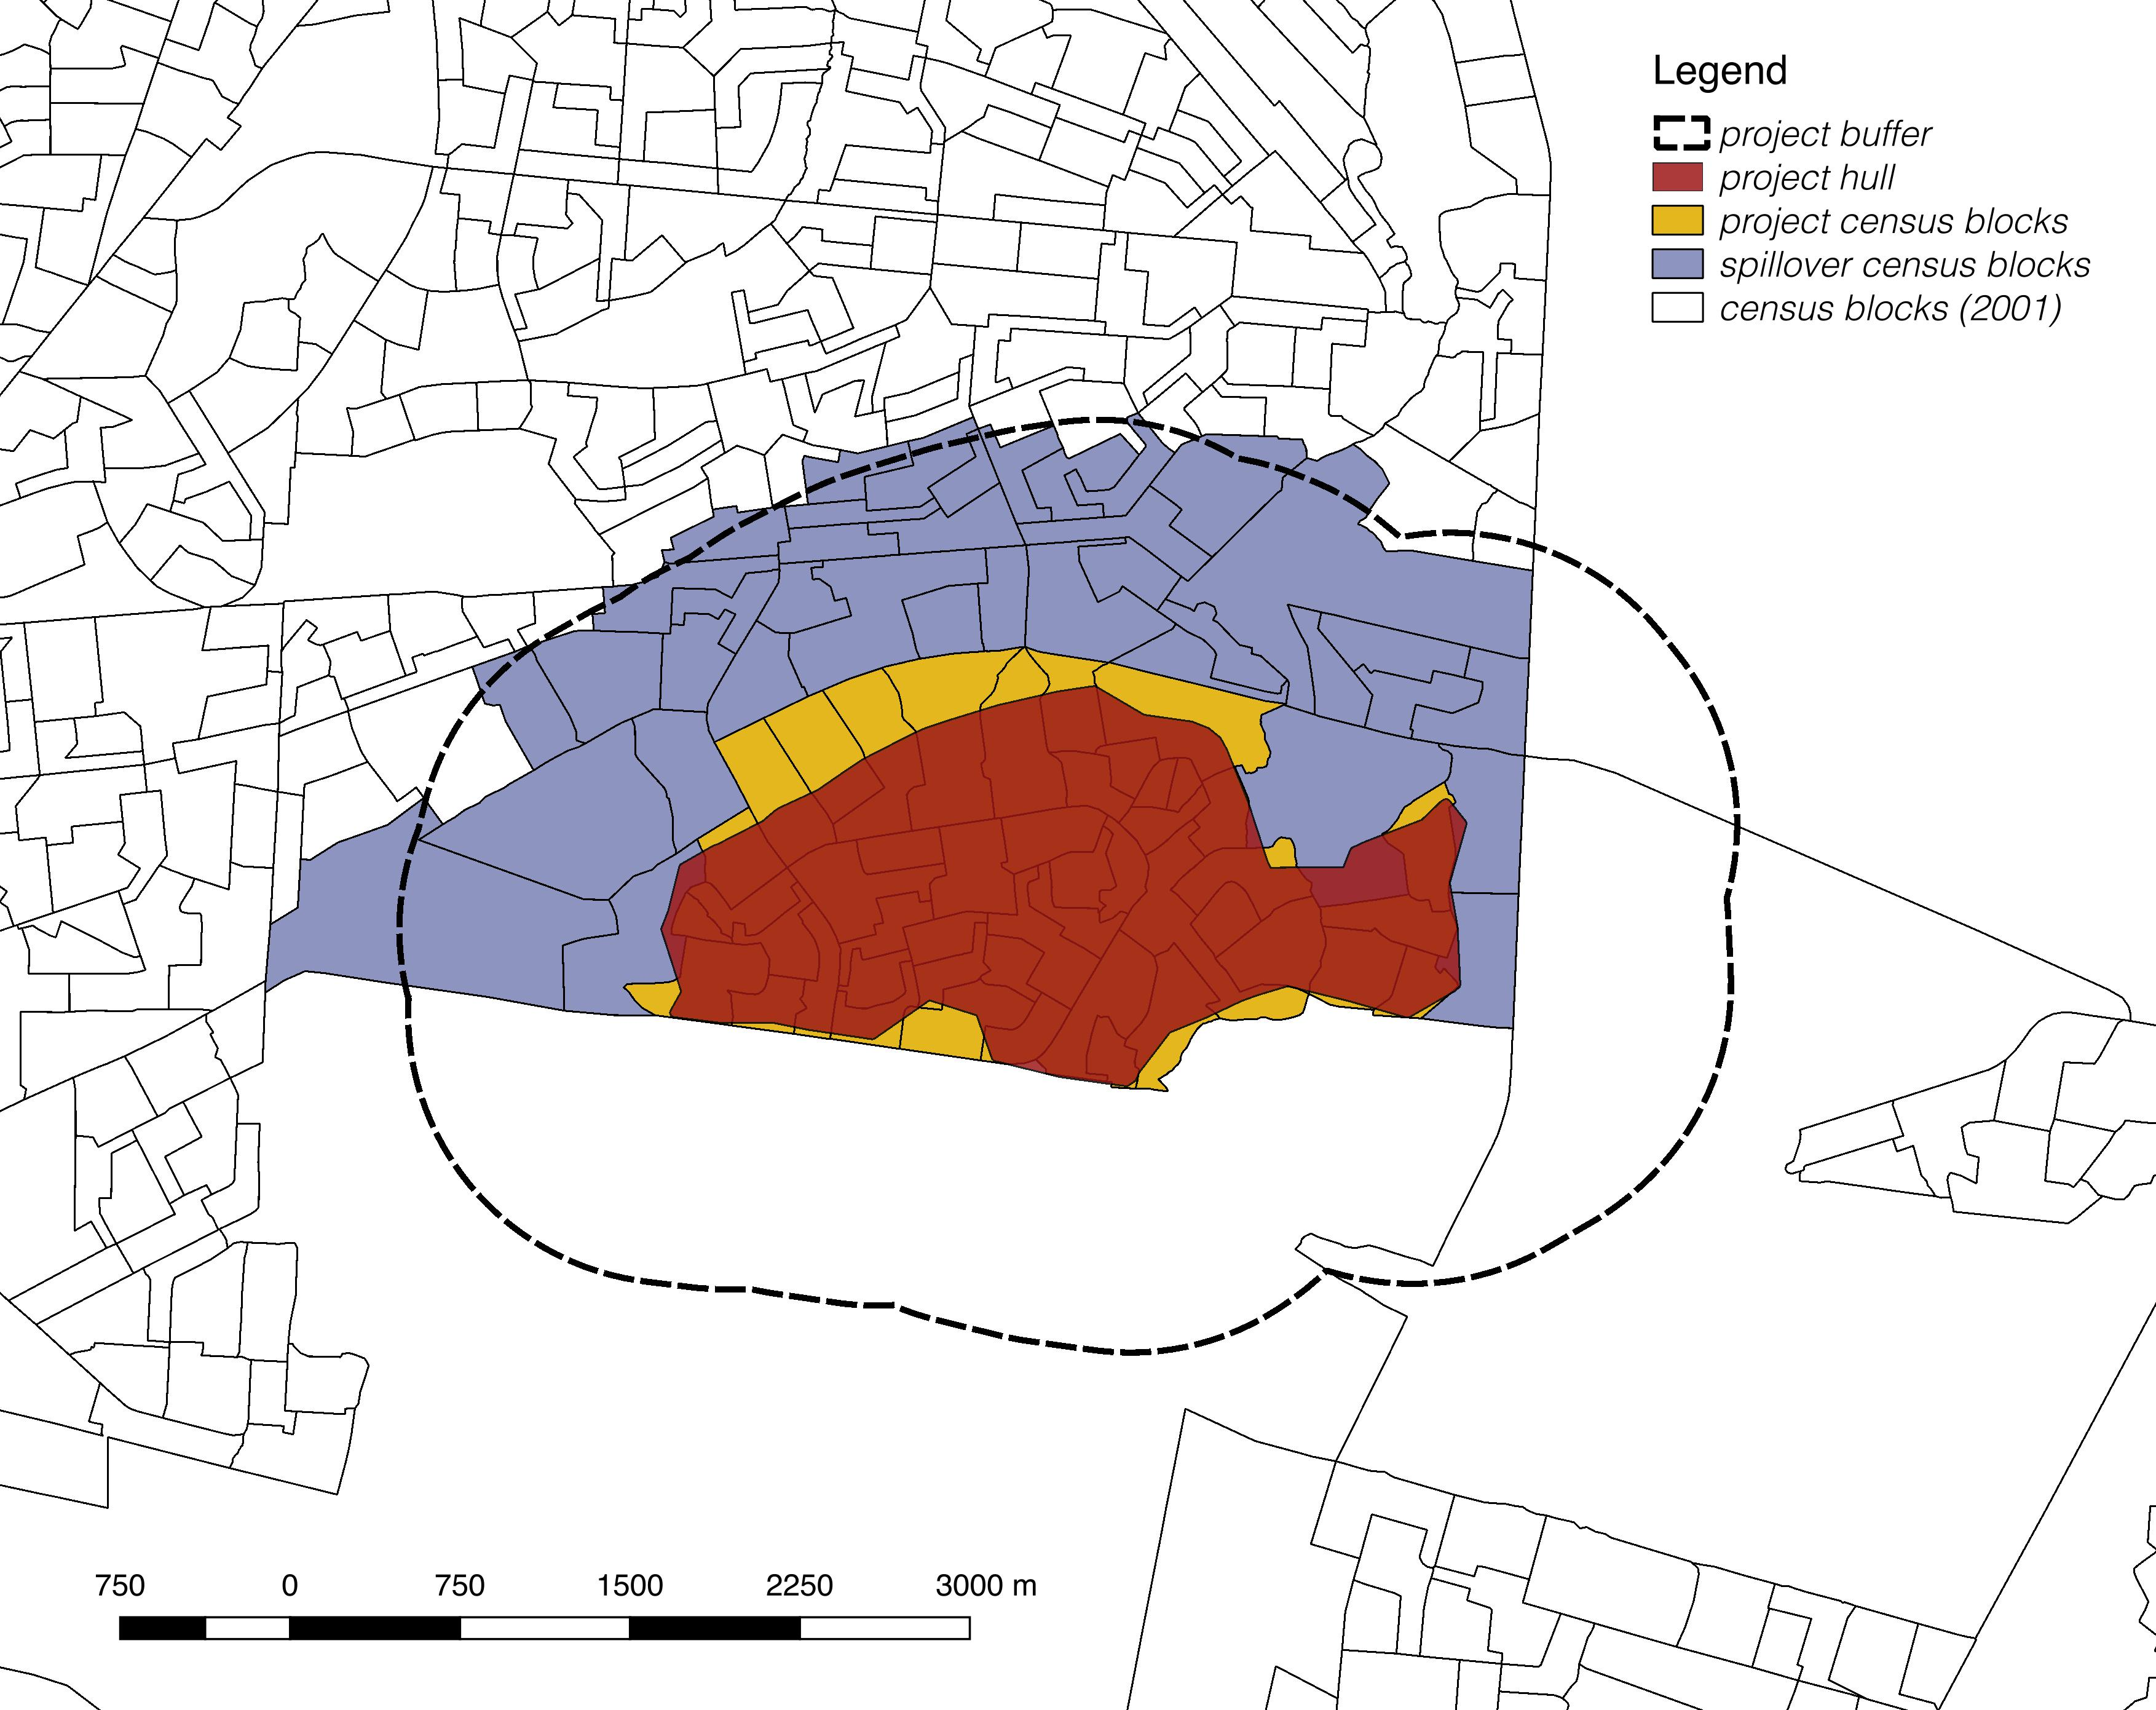
\includegraphics[scale=0.27]{censusmap.jpg}
\vspace{-3mm}
\end{figure}
\end{center}
\end{frame}



%------------------------------------------------

\begin{frame}
\frametitle{Census Descriptives at Baseline (2001)}
\begin{itemize}
    \item Uncompleted project areas have worse outcomes
    \item Spillover areas are comparable
\end{itemize}
\vspace{.1cm}
\centering
\resizebox{\textwidth}{!}{  
\begin{tabu}{lcccc}
 & \multicolumn{2}{c}{Within Project}     & \multicolumn{2}{c}{Outside Project}    \\
 & \multicolumn{2}{c}{($>$30\% Overlap)}  & \multicolumn{2}{c}{($<$30\% Overlap)}   \\
 &  &  &  &  \\ 
 & Completed & Uncompleted & Completed  & Uncompleted  \\
\midrule
 Flush Toilet  & 0.56  & 0.18  & 0.77  & 0.82  \\ 
 &  &  &  &  \\ 
 Piped Water  & 0.21  & 0.07  & 0.41  & 0.36  \\ 
 &  &  &  &  \\ 
 Elec. Cooking  & 0.58  & 0.17  & 0.68  & 0.68  \\ 
 &  &  &  &  \\ 
 Elec. Light  & 0.79  & 0.23  & 0.74  & 0.82  \\ 
 &  &  &  &  \\ 
 Single House  & 0.51  & 0.45  & 0.52  & 0.59  \\ 
 &  &  &  &  \\ 
\midrule
 Observations  & 59,460  & 37,136  & 213,061  & 194,622  \\ 
\bottomrule
\end{tabu}

}
% descriptive_statistics.do program: write_census_hh_table
\end{frame}


%------------------------------------------------



\begin{frame}
\frametitle{Census Difference-in-Differences}
\begin{align*}
Y_{hbtp} \, &= \, \alpha_{1} \, Post_{tp}\,  C_{bp}\,  Project_{bp} \, + \alpha_{2} \, Post_{tp} \, C_{bp} \, Spillover_{bp} \,   \\
&+ \,\theta_1\,  Post_{tp} \, Project_{bp} + \,\theta_2 \, Post_{tp} \, Spillover_{bp}  \,  \\
& + \theta_3\,  C_{bp} \, Spillover_{bp} \, +  \, \theta_4 \, Spillover_{bp} \, +  \lambda_p \, + \, \varepsilon_{hbtp}
\end{align*}

\begin{itemize}
\item $h$: household, $b$: census block, $t$: year (2001, 2011), $p$: project
\item $Post_{tp}$: After project
\item $C_{bp}$: Completed
\item $Project_{bp}$: $>$\%30 overlap
\item $Spillover_{bp}$: $\leq$\%30 overlap
\item $\lambda_p$: Project fixed effect
\end{itemize}

\begin{itemize}
  \item \textbf{Identification}: Counterfactual outcomes for completed projects would have changed in the same way as uncompleted projects.
\end{itemize}


% descriptive_statistics.do program: write_census_hh_table
\end{frame}



%------------------------------------------------



\begin{frame}
\frametitle{Census Differences-in-Differences Estimates}

\resizebox{\textwidth}{!}{  
\begin{tabular}{lcccc} \hline
 & (1) & (2) & (3) & (4)  \\
VARIABLES & Flush Toilet & Piped Water Inside & Electric Cooking & Electric Lighting \\ \hline
 &  &  &  &   \\
Project X Post X Complete & 0.210** & 0.202*** & 0.0679 & -0.0482 \\
 & (0.0824) & (0.0540) & (0.0849) & (0.0998)  \\
 Spillover X Post X Complete & -0.0723* & -0.0464 & -0.130*** & -0.0461 \\
 & (0.0411) & (0.0302) & (0.0449) & (0.0385) \\
    &  &  &  &  \\
    Observations & 1,544,285 & 1,544,285 & 1,544,285 & 1,544,285  \\
R-squared & 0.360 & 0.243 & 0.301 & 0.306  \\ \hline
    &  &  &  &  \\
  & (5) & (6) & (7) & (8) \\
 & Single House & Owns House & No. Rooms & Household Size \\ \hline
   &  &  &  &  \\
Project X Post X Complete  & 0.183*** & -0.0523 & 0.286* & 0.0992 \\
  & (0.0451) & (0.0645) & (0.158) & (0.0915) \\
 Spillover X Post X Complete  & -0.0957** & 0.00820 & -0.102 & -0.00151 \\
 & (0.0374) & (0.0501) & (0.0923) & (0.0462) \\
   &  &  &  &  \\
Observations  & 1,479,342 & 1,496,636 & 1,459,677 & 1,532,866 \\
R-squared  & 0.195 & 0.147 & 0.174 & 0.057 \\
 Project FE & YES & YES & YES & YES \\ \hline
\multicolumn{5}{c}{ Robust standard errors clustered at the project level in parentheses} \\
\multicolumn{5}{c}{ *** p$<$0.01, ** p$<$0.05, * p$<$0.1} \\
\end{tabular}


}
%Project census blocks have $>$30\% project overlap.  Spillover census blocks have $\leq$30\% project overlap.

% descriptive_statistics.do program: write_census_hh_table
\end{frame}







%-------------------- PRICE EFFECTS --------------

\begin{frame}
\frametitle{How do projects affect local housing prices?}
\begin{itemize}
  \item Focus on 1,200m buffers around housing projects
\end{itemize}
\begin{center}
\begin{figure}
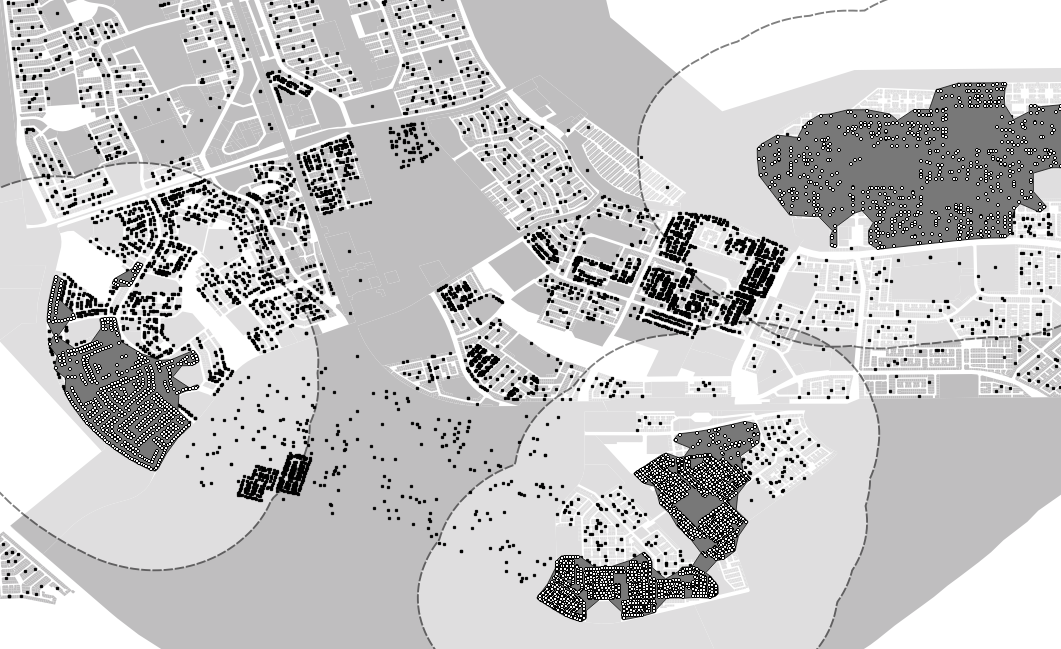
\includegraphics[scale=0.30]{design2.png}
\vspace{-3mm}
\end{figure}
\end{center}
\end{frame}

%------------------------------------------------


\begin{frame}
\frametitle{Housing Price Descriptives}
\begin{center}
\resizebox{.95\textwidth}{!}{  
\begin{tabu}{lccc}
\toprule
 & Outside Buffer & Inside Buffer & Housing Project \\
\midrule
 Purchase Price (Rand)  & 184,199.6  & 205,891.3  & 142,748.8  \\ 
\rowfont{\footnotesize} & [386,165.1]  & [249,590.1]  & [447,771.6]  \\ 
 &  &  &  \\ 
 Plot Size (m3)  & 585.2  & 421.7  & 270.4  \\ 
\rowfont{\footnotesize} & [2,040.3]  & [1,225.7]  & [179.2]  \\ 
 &  &  &  \\ 
 Sold At Least Once  & 0.316  & 0.318  & 0.338  \\ 
 Median Purchase Year  & 2006  & 2006  & 2006  \\ 
 Distance to Project (meters) &  & 373.0  & \\
 \rowfont{\footnotesize} &  & [415.9]  & \\
\midrule
 Observations  & 275,296  & 94,172  & 108,809  \\ 
\bottomrule
\end{tabu}

}
\end{center}
12 Rand = 1 USD
% descriptive_statistics.do program: write_descriptive_table
\end{frame}

%------------------------------------------------


\begin{frame}
\frametitle{Estimating Differences-in-Differences}

\begin{align*}
log P_{itp} \, =& \, \sum_{d=1}^{D} \alpha_d \mathds{1}[dist=d] Post_{tp} \, + \sum_{d=1}^{D} \alpha_d \mathds{1}[dist=d] Pre_{tp} \\
& + \, \gamma_t \, + \, \lambda_p \, + \theta X_{i} + \, \varepsilon_{itp} \\
log P_{itp} \, =& \, \sum_{e=1}^{E} \alpha_j \mathds{1}[time=e] Near_{tp} + \sum_{e=1}^{E} \alpha_j \mathds{1}[time=e] Far_{tp} \\
& \, + \, \gamma_t \, + \, \lambda_p \, + \theta X_{i} + \, \varepsilon_{btp}
\end{align*}

\begin{itemize}
\item $i$: transaction, $t$: year-month, $p$: project
\item $log P_{gtp}$: log price (formal houses)
\item $Near_{tp}$: $<$400m, $Far_{tp}$: $\geq$400m \& $<$1200
\item $Post_{tp}$: 36 months after, $Pre_{tp}$ 36 before
\item $\lambda_p$: project FE, $\gamma_t$: calendar month FE
\end{itemize}


\end{frame}


\begin{frame}
\begin{figure}
\frametitle{Distance Estimates}
%\caption{Price Estimates over Distance}\label{figure:distplot}
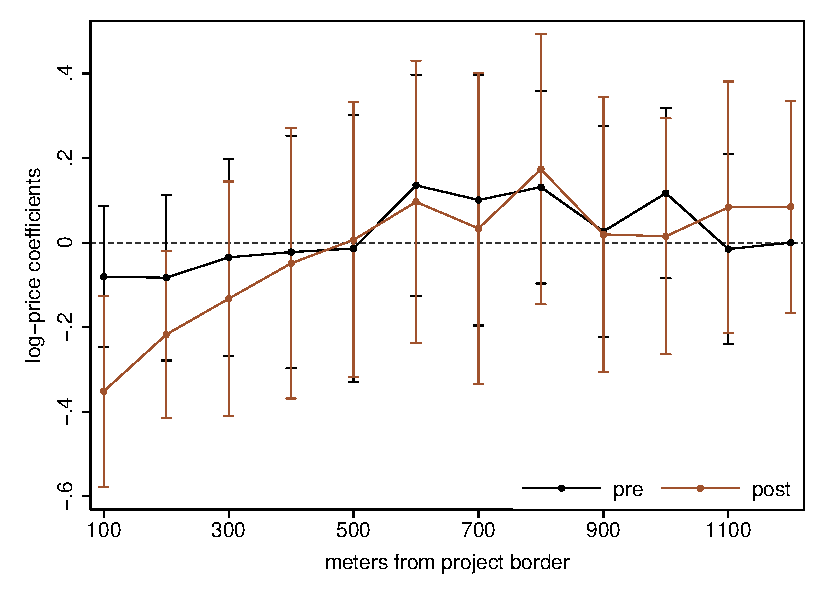
\includegraphics[width=0.5\textwidth,trim={.77cm 0cm .21cm 0cm}]{distplot.pdf}
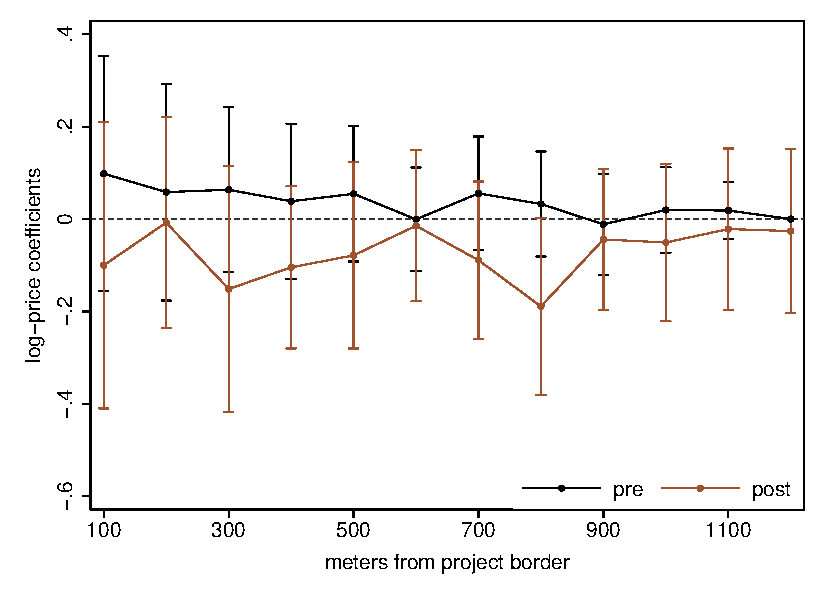
\includegraphics[width=0.5\textwidth,trim={.77cm 0cm .21cm 0cm},clip]{distplot_placebo.pdf}\\
{\color{white}ddd}Completed Projects \hspace{2.4cm} Uncompleted Projects
\end{figure}

\end{frame}



\begin{frame}
\begin{figure}
\frametitle{Time Estimates}
%\caption{Price Estimates over Time}\label{figure:timeplot}
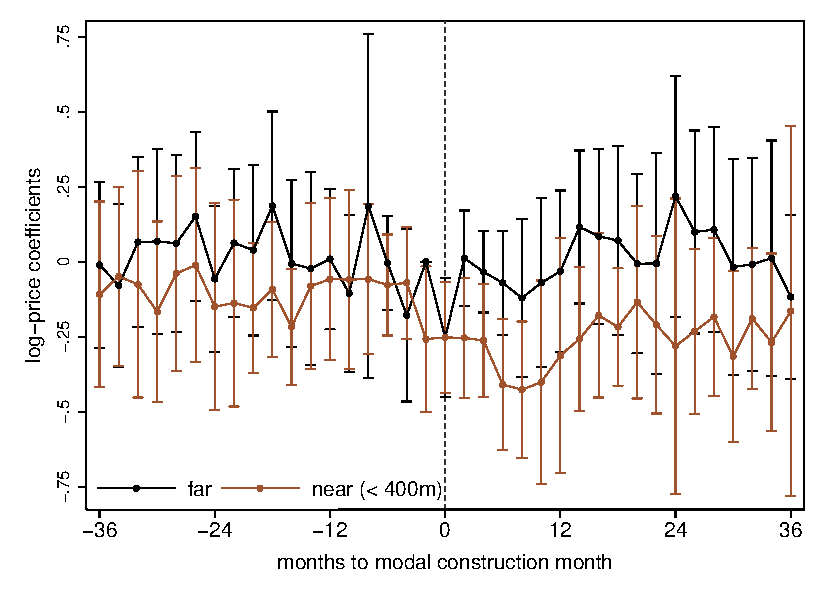
\includegraphics[width=0.5\textwidth,trim={.77cm 0cm .21cm 0cm}]{timeplot.pdf}
   \hfill
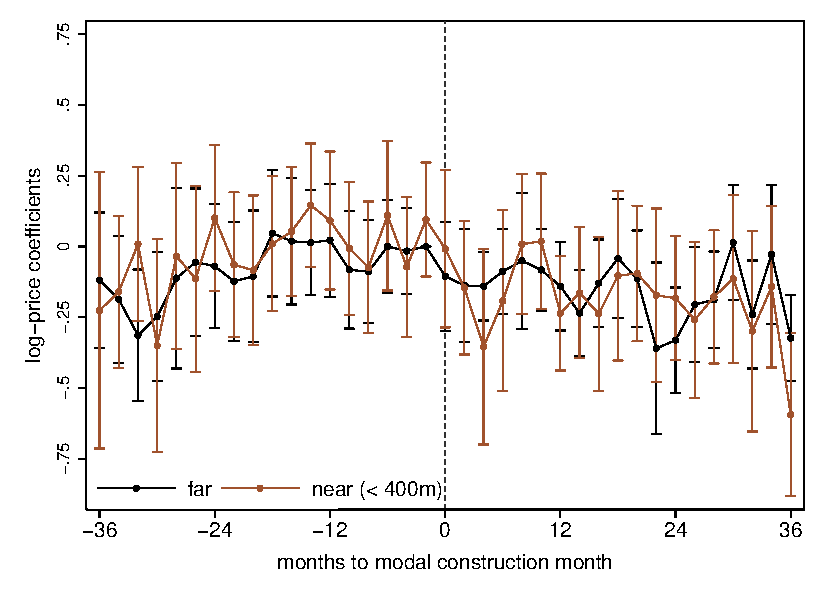
\includegraphics[width=0.5\textwidth,trim={.77cm 0cm .21cm 0cm},clip]{timeplot_placebo.pdf}\\
{\color{white}ddd}Completed Projects \hspace{2.4cm} Uncompleted Projects
\end{figure}
\end{frame}
%------------------------------------------------


\begin{frame}
\frametitle{Regression Analogue}
\begin{center}
\begin{tabular}{lcccc}
& \multicolumn{2}{c}{Completed} & Uncompleted \\
 &   &    &  \\
VARIABLES & Log Price & Log Price  &  Log Price  \\ \hline
   & & &   \\
3 yrs 0-400m & -0.166* & -0.125 &  -0.0664  \\
 & (0.106)  & (0.0892) &  (0.0597) \\
3 yrs 0-400m X In-Situ & & 0.180 &   \\
 &  & (0.289)  &  \\
 &  &  &   \\
Observations & 28,701 & 28,701 &  24,562 \\
R-squared & 0.488 &  0.489 &  0.502 \\
Project FE & YES & YES & YES \\
 Year-Month FE & YES & YES & YES \\ \hline
%\multicolumn{5}{c}{ Robust standard errors in parentheses} \\
%\multicolumn{5}{c}{ *** p$<$0.01, ** p$<$0.05, * p$<$0.1} \\
%\multicolumn{5}{c}{ All control for cubic in plot size. Standard errors are clustered at the project level.} \\
\end{tabular}

\end{center}
In-Situ : top 10\% of informal home density at baseline
\end{frame}


%------------------------------------------------

\begin{frame}
\frametitle{Conclusion and Next Steps}

Conclusions
\begin{itemize}
\item Home quality improves within project footprint but declines nearby
\item Prices in the formal market drop nearby
\item \textbf{Mechanism:} improved services from housing project lowers cost of new slums which generate externalities
\end{itemize}
\vspace{.2cm}

Next Steps
\begin{itemize}
\item Estimate total effect on slum growth
\item Structurally recover externalities from slum density
\item Propose optimal housing policy
\end{itemize}


\end{frame}



%---------------------------------------------
%---------------------------------------------
%--------------   SECOND PAPER  --------------
%---------------------------------------------
%---------------------------------------------

\begin{frame}
\frametitle{}
\centering
{\Large \color{darkred} Subsidized Housing, Household Size, and Child Health} \\
\vspace{.4cm}
\end{frame}

%---------------------------------------------


\begin{frame}
\frametitle{Public Housing and Child Health}

\begin{itemize}
\item \textbf{Question:} How does public housing impact (recipient) child health?
\vspace{.1cm}
  \begin{itemize}
  \item Better materials (Cateneo et al. [2009]; Galiani et al. [2017])
  \vspace{.05cm}
  \item More income (Jacob et al. [2014])
  \vspace{.05cm}
  \item Better neighborhoods (Franklin et al. [2016]; Kling et al. [2005])
  \vspace{.1cm}
  \item \textbf{Relieve overcrowded households}
    \begin{itemize}
      \item More resource investment (more bargaining power for parents)
      \item Less spread of disease
    \end{itemize}
  \end{itemize}

\vspace{.1cm}
\item \textbf{Approach:} Leverage timing of housing projects in South Africa
  \begin{itemize}
    \item Analyze heterogeneous impacts by baseline household size
  \end{itemize}
\vspace{.1cm}

\item \textbf{Findings:}
  \begin{itemize}
    \item Public housing does not affect child health on average
    \item HHs with 6+ members (1) split between new and old houses \\ and (2) experience gains in child health
  \end{itemize}
\end{itemize}

\end{frame}

%---------------------------------------------

\begin{frame}
\frametitle{Theory of Household Splitting and Child Health}
\begin{itemize}
  \item With increasing crowding costs, large households split after receiving a new house
  \vspace{.1cm}
  \item Splitting in response to the program affects child health through
    \begin{enumerate}
      \item Less consumption (to pay for an extra house)
      \item More housing
      \item Less crowding (divide housing/public goods over fewer people)
    \end{enumerate}
\end{itemize}
\end{frame}

%---------------------------------------------

\begin{frame}
\frametitle{Measuring Child Health and Public Housing}

Household-Level Panel Data: (2008, 2010, 2012)
\begin{itemize}
  \item Total: $\sim$5,000 households
  \item This study: 2,038 households (urban, poor) 
  \item Public housing measure: ``Did this household receive a government housing subsidy or any other assistance including RDP housing to obtain this dwelling or any other dwelling?''
  \item 615 households gain housing over the period
\end{itemize}
\end{frame}

%---------------------------------------------

\begin{frame}
\frametitle{Descriptive Statistics at Baseline}
\begin{center}

\begin{tabular}{lccccc}
 & \multicolumn{2}{c}{Control} & \multicolumn{2}{c}{Treated} &  \\
  & mean & N & mean & N & T-Test \\ \hline
 &  &  &  & &  \\
Height (z-score) & -0.879 & 1,698 & -1.056 & 309 & -2.05 \\
Weight (z-score) & -0.324 & 1,579 & -0.436 & 267 & -1.13 \\
Child Health & 1.815 & 3,093 & 1.715 & 643 & -2.46 \\
Household Size & 5.127 & 11,080 & 5.266 & 2,070 & 2.32  \\
Children & 2.176 & 11,080 & 2.389 & 2,070 & 5.16  \\
Rooms & 3.723 & 10,657 & 3.511 & 2,006 & -4.80 \\
Piped Water & 0.538 & 11,080 & 0.505 & 2,070 & -2.74 \\
Flush Toilet & 0.450 & 11,080 & 0.472 & 2,070 & 1.88 \\
Market Value & 19,009 & 3,714 & 19,681 & 735 & 0.93 \\
Income (month) & 3,704 & 10,569 & 2,441 & 1,943 & -8.05 \\
 &  &  &  &    \\ \hline
%\multicolumn{7}{c}{ Child Health ranges from 1 Healthy to 5 Sick.} \\
\end{tabular}


\end{center}
\end{frame}






%---------------------------------------------

\begin{frame}
\frametitle{Empirical Approach: Estimate with First-Differences}

\begin{align*}
\Delta Y_{ijpt}  =& \, \beta_0 + \beta_1 \Delta Proj_{ijpt} + \beta_2 \Delta X_{ijpt} + \Delta \gamma_{pt} + \Delta \varepsilon_{ijpt} \\
&\\
\Delta Y_{ijpt}  =& \, \alpha_0 + \alpha_1 Large_{ijpt-1} + \alpha_2 \Delta  Proj_{ijpt} + \alpha_3 \Delta Proj_{ijpt} \times Large_{ijpt-1} \\ 
 &+ \alpha_4 \Delta X_{ijpt}  + \Delta \gamma_{pt} + \Delta \varepsilon_{ijpt} 
\end{align*}
\begin{itemize}
  \item $i$: individual, $j$: household, $p$: province, $t$: year
  \item $Proj_{ijpt}$: housing project
  \item $Large_{ijpt-1}$: 6+ HH members in the previous year
  \item $X_{ijpt}$: household/individual controls
  \item $\gamma_{pt}$: province time trends
\end{itemize}
\begin{itemize}
  \item \textbf{Identification}: Counterfactual outcomes for treated individuals would have changed in the same way as untreated individuals.
\end{itemize}
\end{frame}

%---------------------------------------------

\begin{frame}
\frametitle{Impacts on Housing Quality}
\resizebox{\textwidth}{!}{  
\begin{tabular}{lcccccc} 
% & (1) & (2) & (3) & (4) & (5) & (6) \\
 & Piped Water & Flush Toilet & Brick Walls & Refuse Service & Mkt Value & Rooms \\ \hline
 &  &  &  &  &  &  \\
Proj & 0.160*** & 0.137*** & 0.178*** & 0.0445* & 5,577* & 0.0172 \\
 & (0.0417) & (0.0460) & (0.0393) & (0.0264) & (3,248) & (0.0932) \\
ProjxLarge t-1 & -0.109 & 0.00559 & -0.0823 & -0.00740 & 2,902 & 0.0396 \\
 & (0.0865) & (0.0887) & (0.0801) & (0.0564) & (8,554) & (0.181) \\
Proj t-1 & 0.0506 & -0.0530 & -0.0361 & -0.000981 & -1,540 & 0.166 \\
 & (0.0578) & (0.0633) & (0.0509) & (0.0382) & (3,176) & (0.179) \\
Proj t-1xLarge t-1 & 0.0696 & 0.0190 & 0.0211 & -0.0224 & -526.3 & -0.0955 \\
 & (0.118) & (0.131) & (0.104) & (0.0914) & (13,938) & (0.349) \\
Large t-1 & 0.0330 & -0.0338 & -0.00299 & -0.0214 & -120.9 & -0.0210 \\
 & (0.0355) & (0.0432) & (0.0356) & (0.0264) & (6,368) & (0.116) \\
 &  &  &  &  &  &  \\
Observations & 8,421 & 8,421 & 8,421 & 7,621 & 1,165 & 7,411 \\
R-squared & 0.047 & 0.079 & 0.062 & 0.034 & 0.115 & 0.044 \\ \hline
% Treated Area & Over 5 & Over 5 & Over 5 & Over 5 & Over 5 & Over 5 \\ \hline
\end{tabular}

}
\end{frame}

%---------------------------------------------


\begin{frame}
\frametitle{Overall Impacts on Health}
\resizebox{\textwidth}{!}{  
\begin{tabular}{lcccc} 
% & (1) & (2) & (3) & (4) & (5) & (6) \\
  & Height (z-score)  & Weight (z-score)  & Illness & Health \\ \hline
  &  &  &  &  \\
Proj  & 0.0270  & -0.0792 & 0.0221 & 0.0661 \\
  & (0.0636)  & (0.0837) & (0.0179) & (0.0664) \\
Proj t-1  & 0.0548  & -0.00209 & -0.00352 & -0.00870 \\
  & (0.121)  & (0.151) & (0.0303) & (0.130) \\
   &  &  &  &  \\
Observations  & 413 & 445 & 1,120 & 1,122 \\
R-squared  & 0.164 & 0.183 & 0.597 & 0.548 \\
%Treated Area & Full Sample & Over 5 & Full Sample & Over 5 & Over 5 & Over 5 \\
 Mean  & -0.869 & -0.271 & 0.0618 & 1.666 \\ \hline
\end{tabular}

}
\end{frame}


\begin{frame}
\frametitle{Impacts on Household Size}
\begin{center}  
  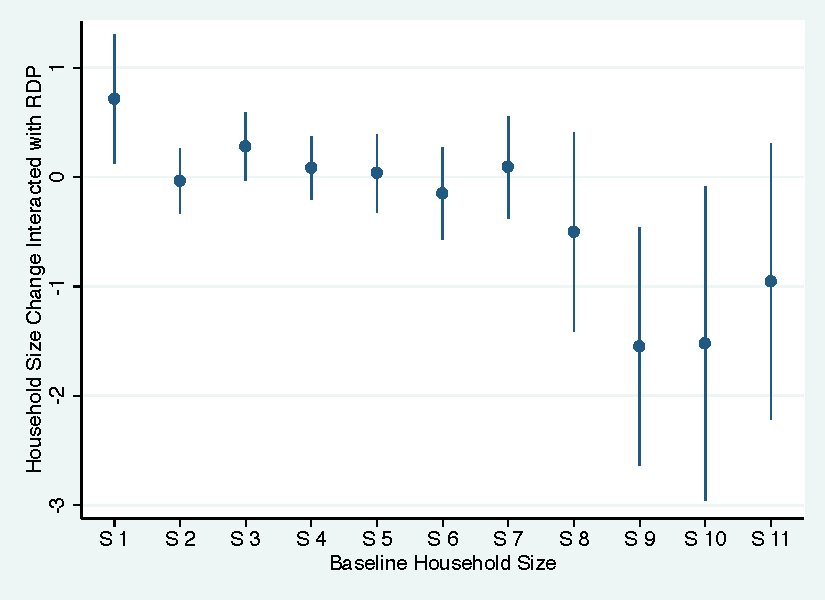
\includegraphics[scale=.75]{size_ch.pdf}
\end{center}
\end{frame}

\begin{frame}
\frametitle{Effects on Child Height and Weight according to Baseline Household Size}
\begin{center}
\hspace*{-10mm}
  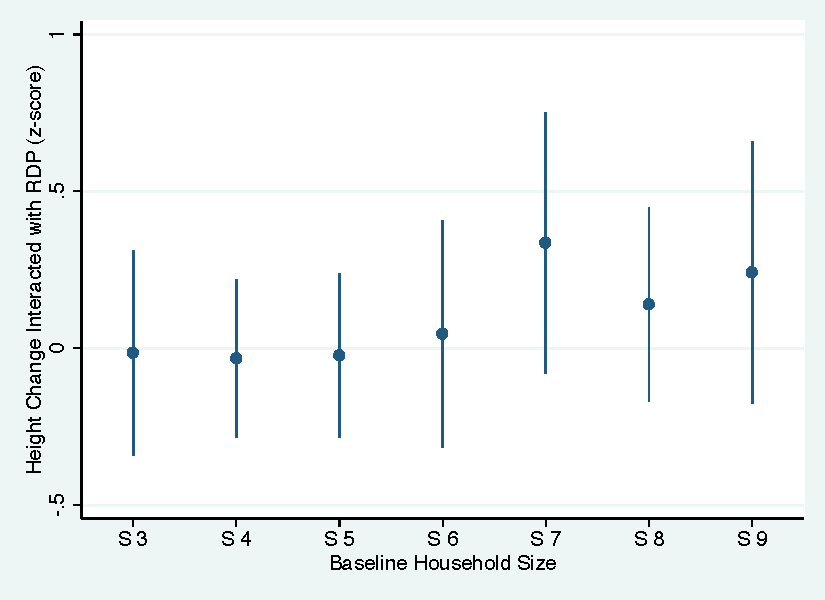
\includegraphics[scale = 0.49]{height_ch.pdf}
  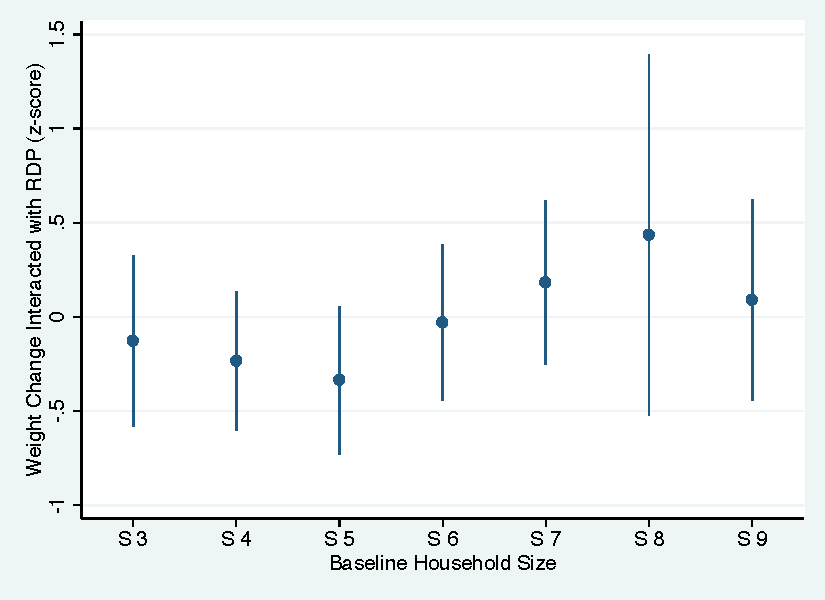
\includegraphics[scale = 0.49]{weight_ch.pdf}
\end{center}
\end{frame}

\begin{frame}
\frametitle{Household Size and Health Impacts}
\resizebox{\textwidth}{!}{  
\begin{tabular}{lccccccc} \hline
 & (1) & (2) & (3) & (4) & (5) & (6) & (7) \\
 & HH Size & Height  & Height   & Weight  & Weight  & Health  & Ill  \\ \hline
 &  &    &  &  & & & \\
Proj & 0.0423  & 0.0102 & 0.000920 & -0.189* & -0.205* & 0.0744 & 0.00461  \\
  & (0.0766) & (0.0725) & (0.0717)  & (0.105) & (0.106) & (0.0810) & (0.0204) \\
ProjxLarge t-1  & -0.787*** & 0.130 & 0.225*  & 0.371* & 0.395** & -0.0439 & 0.0511 \\
 & (0.237) & (0.134) & (0.130)  & (0.202) & (0.199) & (0.154) & (0.0481) \\
Proj t-1  & 0.0591 & 0.0719 & -0.0113 & 0.0173 & 0.0285  & -0.0488 & 0.00972 \\
 & (0.101)  & (0.133) & (0.140)  & (0.153) & (0.161)  & (0.137) & (0.0374) \\
Proj t-1 x Large t-1  & -0.479 & -0.130 & 0.0368  & -0.619 & -0.679  & 0.120 & -0.0725* \\
 & (0.438) & (0.264) & (0.293)  & (0.474) & (0.458)  & (0.355) & (0.0395) \\
Large & -0.505***  & -0.0608 &   & -0.186** &  &  0.0697 & -0.00440   \\
 & (0.102)   & (0.0654) &  &  (0.0869) &  & (0.0684) & (0.0195)  \\
 &  &    &  & & &   \\
Observations & 9,898 & 534 & 534 & 576 & 576  & 1,122 & 1,120\\
R-squared & 0.172 & 0.202 & 0.237 & 0.218 & 0.253 & 0.547 & 0.599 \\
Time x Prov FE   & YES & YES & NO & YES & NO & YES & YES \\
Time x Prov x Large FE & NO  & NO & YES & YES & NO & NO & NO \\
%Treated Area & Full Sample & Full Sample & Over 5 & Full Sample & Full Sample & Over 5 \\
Mean & 5.127 & -0.967 & -0.967  & -0.262 & -0.262  & 1.731 & 0.0728  \\
 F-Stat: Proj+ProjxLarge=0 & & 1.429 & 3.823  & 1.375 & 1.537 & &  \\ \hline
\multicolumn{8}{c}{ All health regressions control for lagged quartiles in outcomes} \\ 
\end{tabular}

}
\end{frame}

\begin{frame}
\frametitle{Conclusion}


Additional findings
\begin{itemize}
  \item No change in HH income
  \item Fewer people per room
  \item Improvements in domestic violence and nearby drug use
  \item Expenditure shifts from non-food towards food
  \item ``Left out'' HH members move to slums, work more, and send remittances to family
\end{itemize}
\vspace{.1cm}
Conclusions
\begin{itemize}
  \item Both mechanisms -- (1) less disease spread and (2) better bargaining for children -- may contribute to child health improvements for crowded households at baseline
\end{itemize}

\vspace{.1cm}
Next Steps
\begin{itemize}
  \item Improve definition of project area using administrative data
  \item Include most recent wave of panel
\end{itemize}

\end{frame}






%---------------------------------------------
%---------------------------------------------
%--------------   THIRD  PAPER  --------------
%---------------------------------------------
%---------------------------------------------

\begin{frame}
\frametitle{}
\centering
{\Large \color{darkred} Optimal Pricing and Informal Sharing: \\ \vspace{.1cm} Evidence from Piped Water in Manila} 
\end{frame}

%---------------------------------------------


\begin{frame}
\frametitle{Pricing public utilities}
\begin{itemize}
\item Access to public utilities {\small -- piped water, electricity, mobile phones} \\
$\rightarrow$ large economic benefits  \\
        {\footnotesize{ {(health, time/cost savings, employment, etc.)}  }}\\
%%%       {\footnotesize{ \textcolor{gr}{Gamper-Rabindran et al. [2010], Galiani et al. [2005], \\ Dinkelman [2011], Bjorkegren [2017]}  }}\\ 

  \vspace{.3cm}     
\item Govts set prices to increase access while covering costs
  \vspace{.1cm}
  \begin{itemize}
    \item Low fixed prices per connection
    \item High marginal prices per unit (increasing)
%  \pause    
    \vspace{.1cm}
    \item \textbf{Assume} one household per connection
  \end{itemize}
  \vspace{.2cm}
%  \pause
\item But people often share connections informally
\vspace{.1cm}
  \begin{itemize}
    \item High (increasing) marginal prices tax shared connections \\ 
$\rightarrow$ may lower access and welfare
  \end{itemize}
  \vspace{.1cm}
%  \pause
  \vspace{.3cm}
\item \textbf{Question:} What is the optimal pricing policy \\
\hspace{2.4cm} when people share connections?
\end{itemize}
\end{frame}


%---------------------------------------------


\begin{frame}
\frametitle{Pricing piped water in Manila, Philippines}
\begin{itemize}
% \item \textbf{Context:} Water provision in Manila, Philippines
%   \vspace{.5cm}
\item \textbf{Question:} What is the optimal pricing policy \\
\hspace{2.4cm} when people share connections?
\vspace{.2cm}
%\begin{itemize}
  \item Key inputs: 1) demand, 2) sharing costs, 3) production costs

\vspace{.3cm}

  \item \textbf{Approach:} source and usage reveal sharing costs and demand
%\pause
\vspace{.3cm}
  \item \textbf{New Data:} estimate using transaction panel with sharing survey
      \vspace{.1cm}
    \begin{itemize}
      \item Sudden price changes identify demand
      \item Quasi-experiment identifies sharing costs
    \end{itemize}
%\pause
\vspace{.3cm}
  \item  \textbf{Policy:} optimum $\rightarrow$ high fixed and low marginal prices
      \vspace{.1cm}
    \begin{itemize}
    % \item High fixed price and low marginal price
    %   \vspace{.05cm}
      \item Welfare gain: 70\unskip\% of consumer surplus (0.6\unskip\% of HH inc)
        \vspace{.05cm}
      \item Greater sharing $\rightarrow$ improves access
    %   \vspace{.1cm}
    \end{itemize}
    \vspace{.2cm}
  \item Also consider social pricing and pricing without sharing  
\end{itemize}
\end{frame}
%---------------------------------------------


\begin{frame}
\frametitle{ Contribution to the literature}

\begin{itemize}
  \item \textcolor{navyblue}{Theory:} Ramsey (1939); Auerbach and Pellechio (1978); Feldstein (1972)
  \item \textcolor{navyblue}{Demand estimation:} Moffitt (1986); Borenstein (2009); \\ Olmstead (2009)
  \item \textcolor{navyblue}{Development applications:} Szab\'{o} (2015); Diakit\'{e} et al. (2009); McRae (2014); Devoto et al. (2012)
  % \vspace{.4cm}
\end{itemize}
\vspace{.1cm}
Contributions
\vspace{.1cm}
\begin{itemize}
  \item \textcolor{blue}{Model not only ``intensive'' usage, but also ``extensive'' source} 
  \begin{itemize}
    \item \textcolor{blue}{Endogenous sharing}
  \end{itemize}
  \item \textcolor{blue}{Estimate with micro-data for a large metro-area}
  \end{itemize}
%\vspace{.2cm}
%\item Barriers in connecting to piped water
%\vspace{.1cm}
% \begin{itemize}
%   \item Devoto et al. (2012); Ashraf et al. (2016); Kayaga and Franceys (2007)  {\footnotesize (govt fees, proving land tenure, credit constraints, etc.)}
%     \vspace{.2cm} 
%   \item \textcolor{blue}{Provide a structural estimate of hard-to-measure barriers}
% \end{itemize}
%\end{itemize}
\end{frame}

\begin{frame}
\frametitle{Main Findings}

Model and Estimation
\begin{itemize}
  \item Sharing water lets households trade a lower fixed cost for a higher marginal cost
  \item Households are price sensitive (elasticity of 0.5)
  \item Households face high ``hard-to-measure'' fixed costs \\
   (repairs, permitting, land tenure, etc.)
\end{itemize}

\vspace{.2cm}

Policy Takeaways
\begin{itemize}
  \item Simple two-part tariff (high fixed price/low marginal price)
    \begin{itemize}
      \item Large users enjoy low marginal price
      \item Small users also enjoy low marginal price through their neighbors
      \item Non-linear pricing has negligible impacts on welfare
    \end{itemize}
  \item Setting marginal price above marginal cost can mitigate free-riding
\end{itemize}


\end{frame}


\begin{frame}
\frametitle{Next Steps}

\begin{itemize}
  \item Extensive margin of where to get water may respond to price changes over time
  \item Linearity of demand
  \item Optimal policy is far out of sample
\end{itemize}

\end{frame}



\begin{frame}
\begin{center}
\textcolor{navyblue}{\Large \bf Thank You! } 
\end{center}
\end{frame}







%------------------------------------------------


%\begin{frame}
%\frametitle{Conceptual Framework}
%
%How would housing projects spillover to neighborhood outcomes?
%\vspace{.2cm}
%\begin{enumerate}
%  \item \textbf{Amenity Effect:} Upgrading housing stock/services
%    \begin{itemize}
%        \item Increase value of neighboring homes (Rossi-Hansberg [2010])
%    \end{itemize}
%\vspace{.2cm} 
%
%  \item \textbf{Crowd-In Slums:} Reduce costs of informal housing
%    \begin{itemize}
%        \item Overburden services, health/crime externalities
%        \item Reduce value of nearby houses
%    \end{itemize}
%\vspace{.2cm}
%
%  \item \textbf{Demographic Effect:} New people in the neighborhood
%    \begin{itemize}
%        \item Taste-based discrimination (Diamond and McQuade [2016])
%    \end{itemize}
%\end{enumerate}

%\begin{enumerate}
%  \item Housing externalities  {\small (Rossi-Hansberg [2010]) }
%    \begin{itemize}
%      \item Home value depends on the quality of neighboring homes
%      \item ie. informal dwellings have poor sanitation
%    \end{itemize}
%\vspace{.1cm}
%  \item Demographic externalities
%    \begin{itemize}
%      \item Taste-based discrimination
%      \item Overcrowding $\rightarrow$ crime/health externalities
%    \end{itemize}
%\vspace{.1cm}
%  \item Access to public goods (water, sewer, road infrastructure)
%\end{enumerate}
%\end{frame}



\begin{frame}
\frametitle{Identifying Housing Projects} 
\label{dataappendix}

\begin{tikzpicture}[overlay]

\onslide<1->\node[overlay,anchor=west,align=left] at (0, 2.5) {    \begin{minipage}{1\textwidth} {\begin{enumerate}
  \item \textbf{Seller Identity:} match government names and housing authorities in seller-names from transactions 
\end{enumerate}}\end{minipage}};

\onslide<2->\node[overlay,anchor=west,align=left] at (0, 1.5) {    \begin{minipage}{1\textwidth} { 
\begin{enumerate}
  \setcounter{enumi}{1}
  \item \textbf{Subsidy Value:} exclude purchase prices R50,000 above subsidy value ($<$4\% of remaining transactions)
\end{enumerate}}\end{minipage}};

\onslide<3->\node[overlay,anchor=west,align=left] at (0, .5) {    \begin{minipage}{1\textwidth} { 
\begin{enumerate}
  \setcounter{enumi}{2}
  \item \textbf{Pre-Existing Formal Dwellings:} exclude land plots with formal structures in 2001 building census (31\% of remaining transactions)
\end{enumerate}}\end{minipage}};

\onslide<4->\node[overlay,anchor=west,align=left] at (0, -.5) {    \begin{minipage}{1\textwidth} { 
\begin{enumerate}
  \setcounter{enumi}{3}
  \item \textbf{Spatial Clustering:} collect nearby houses into projects with density-based clustering algorithm
\end{enumerate}}\end{minipage}};

\onslide<5->\node[overlay,anchor=west,align=left] at (0, -1.5) {    \begin{minipage}{1\textwidth} { 
\begin{enumerate}
  \setcounter{enumi}{4}
  \item \textbf{Temporal Clustering:} include clusters with $>$50\% of transactions during modal year (\%50 of clusters)
\end{enumerate}}\end{minipage}};

\onslide<5->\node[overlay,anchor=west,align=left] at (0, -2.6) {    \begin{minipage}{1\textwidth} { 
\begin{itemize}
  \item Overlaps well with completed projects from admin. data
\end{itemize}}\end{minipage}};



\onslide<1>\node[overlay,anchor=west,align=left] at (0, -1) {
\begin{minipage}{1\textwidth} { 
\begin{figure}
\caption{Top 5 Seller Names}
\begin{tabu}{lc}
\toprule
 Seller Name & Observations \\
\midrule
City Of Johannesburg Metropolitan Municipality & 29,087  \\
City Of Johannesburg & 27,672  \\
City Of Tshwane Metropolitan Municipality & 24,780  \\
Ekurhuleni Metropolitan Municipality & 21,758  \\
Gauteng Provincial Housing Advisory Board & 13,058  \\
{\bf Total Observations }& {\bf 549,704}  \\
\bottomrule
\end{tabu}
 
\end{figure}
}\end{minipage}
} ;
% descriptive_statistics.do   program: write_biggest_sellers


\onslide<2>\node[overlay,anchor=west,align=left] at (0, -2) { 
\begin{minipage}{1\textwidth} { 
\begin{figure}
\caption{Purchase Price Densities}
 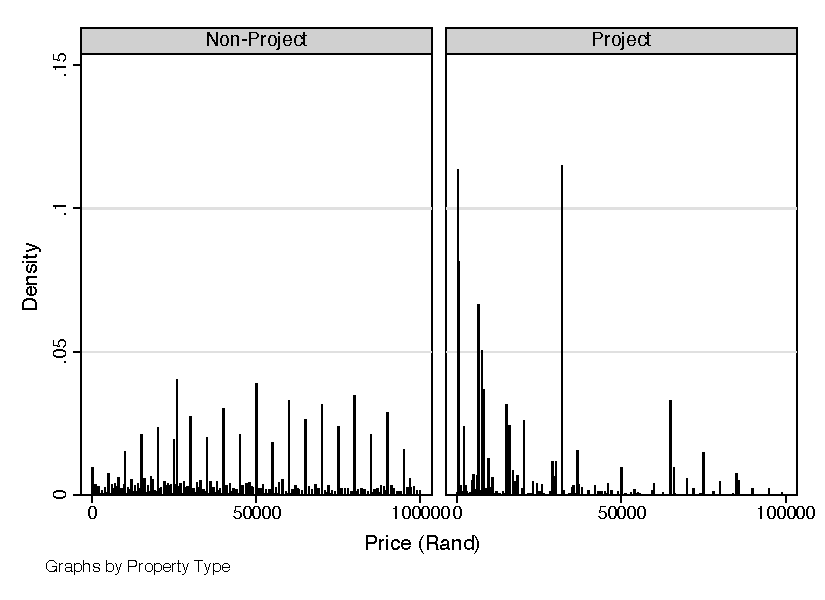
\includegraphics[scale=.5]{price_histogram.pdf} 
\end{figure}
}\end{minipage} 
} ;
% descriptive_statistics.do   program: write_price_histogram


\onslide<4>\node[overlay,anchor=west,align=left] at (2, -2.8) {  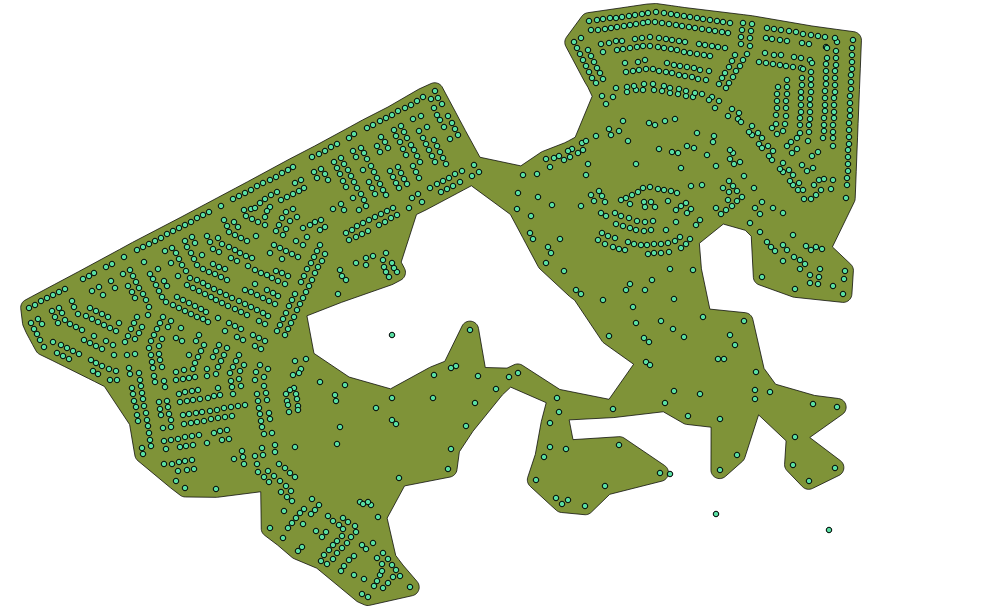
\includegraphics[scale=.16]{rdp_conhull_pic.png}  };
% generated from QGIS


\end{tikzpicture}

\hyperlink{data}{\beamerbutton{return}}

\end{frame}




\end{document} 
